\documentclass{article}
\usepackage{graphicx}
\usepackage[utf8]{inputenc}
\usepackage[fleqn]{amsmath}
\usepackage{titling}
\usepackage{graphicx,wrapfig,lipsum}
\usepackage{amssymb}
\usepackage{listings}
\usepackage[font=small,labelsep=none]{caption}
\usepackage{hyperref}
\usepackage{caption}

\setlength{\droptitle}{-10em}
\setlength\parindent{0pt}

\title{Project 3}\vspace{-3ex}
\author{Benedicte Allum Pedersen, Emil Heland Broll\\ Fredrik Oftedal Forr}
\date{\vspace{-5ex}}

\begin{document}
\maketitle

\section*{Abstract}
	We have computed the integral for the expectation value of the correlation energy between to electrons in a helium atom by using Gauss-Legendre and Gauss-Laguerre quadrature as well as Monte Carlo integration. We experienced that the brute force methods gave a less satisfactory resulst compared to the methods that required some more thinking and adaptation of the integrand and the approximated limits. The exact, analytical value of the integral should be $0.192765$. The best value we got from Gauss-Legendre was $0.192651$, while the best value from Gauss-Laguerre was $0.194779$. We also experienced that Gauss-Laguerre gave better results when we increased the number of integration points, while this was not the case for Gauss-Legendre.
	The Monte Carlo brute force method improved the precision when increasing the number of integration points, and the improved Monte Carlo method followed the same general trend, but with some outliers.
	The fastest, most precise method was the [...]

\section*{Introduction}
	In this report we will give a brief rundown on different numerical integration methods. The methods we will go through are Gauss-Legendre and Gauss-Laguerre quadrature as well as Monte Carlo integration. We will also try to improve the different methods and find the strengths and weaknesses of the methods compared to each other.\\
	We will explain the various integration methods, results from our integrations and a discussion of the results, and finally a conclusion on how the different methods perform and compare to each other.\\

	The integral we will study is the six-dimensional integral determining the ground state correlation energy between two electrons in a helium atom.\\

	The single-particle wave function for an electron $i$ in the $1s$ state in a hydrogen atom is as follows:

	\begin{flalign*}
		\psi_{1s}(\textbf{r}_i)= e^{- \alpha r_i}
	\end{flalign*}

	where $\textbf{r}_i = x_i \textbf{e}_x + y_i \textbf{e}_y + z_i \textbf{e}_z$, and the value $r_i$ is given by:

	\begin{flalign*}
		r_i = \sqrt{x_i^2 + y_i^2 +z_i^2}
	\end{flalign*}

	We set $\alpha = 2$ which corresponds to the charge of the helium atom, Z = 2. We assume that the wave function for each electron in the helium atom can be modelled like the single-particle wavefunction above. The wavefunction for two electrons is then given by the product of two single-particle wavefunctions:

	\begin{flalign*}
		\Psi(\textbf{r}_1, \textbf{r}_2) = e^{-\alpha(r_1 + r_2)}
	\end{flalign*}

	We need to solve the intergral for the expectation value of the correlation energy between the two electrons:

	\begin{flalign*}
		\left<\frac{1}{|\textbf{r}_1 - \textbf{r}_2|}\right> = \int_{-\infty}^{\infty} e^{-\alpha(r_1 + r_2)} \frac{1}{|\textbf{r}_1 - \textbf{r}_2|} d\textbf{r}_1 d\textbf{r}_2
	\end{flalign*}

	The exact value of this integral is $5\pi^2/16^2 = 0.192765$.


\section*{Method}
	In this project we are using C++ to program the numerical algorithms for solving the integrals.

	\subsection*{Our integrand}
		In order to perform the integration, we need to know how to approximate the infinite limits of the integral. To do this, we plot the wave function for the electrons in the Helium atom in figure \ref{fig:wavefunc}. From this plot we can tell that the integral converges to zero for $x < -2$ and $ x > 2$. Therefore the integral would not need to be evaluated outside of those values of x, as the total contribution from the area outside of that interval would be negligible.
		\begin{figure}[hbt]
		\begin{center}
				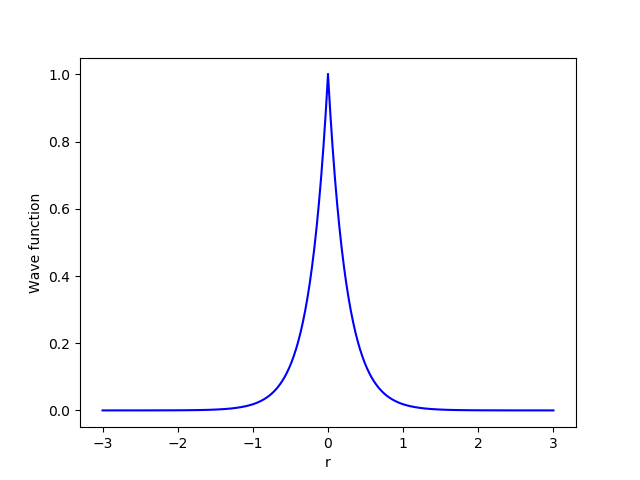
\includegraphics[width=200px]{Wave_func.png}
				\caption{: Plot of the wave function for to electron in a Helium atom.}
				\label{fig:wavefunc}
		\end{center}
		\end{figure}

	\subsection*{Gaussian quadrature}
		The first method we will look at is Gaussian quadrature. To compute the integral numerically we approximate by discretising our variables:
		\begin{flalign*}
			I = \int_{a}^{b} f(x) dx = \int_{a}^{b} W(x)g(x) dx \approx \sum_{i=1}^{N} \omega_i f(x_i)
		\end{flalign*}

		Unlike other more basic methods for numerical integrations where the mesh points $x_i$ are equidistantly spaced, the mesh points in the Gaussian quadrature are not equidistantly spaced. In the sum above, the $w_i$ corresponds to the weights. Gaussian quadrature uses orthonogonal Legendre- and Laguerre-polynomials to obtain the mesh points and weights.\\

		\textbf{Gauss-Legendre} is a brute-force method, and in order to obtain the value of the integral using this method we have to set up the mesh points and weights that corresponds to some finite integrations limits [a, b]. To set up the mesh points and weights we haved used the function $gauleg$ from professor Morten Hjorth-Jensen's \href{https://github.com/CompPhysics/ComputationalPhysics/blob/master/doc/Projects/2019/Project3/CodeExamples/exampleprogram.cpp}{example program}. We then need to apporoximate our integration limmits $-\infty$ and $\infty$ with $-\lambda$ and $+\lambda$.\\

		While the Legendre polynomials are defined for $x \in [-1, 1]$ the \textbf{Laguerre polynomials} are defined for $x \in [0, \infty)$. To improve our result, we rewrite the integral by changing to spherical coordinates:
		\begin{flalign*}
			d\textbf{r}_1d\textbf{r}_2 = r_1^2dr_1r_2^2dr_2dcos(\theta_1)dcos(\theta_2)d\phi_1d\phi_2
		\end{flalign*}

		Thus the integral becomes:
		\begin{flalign*}
			I = \int_0^\infty r_1^2dr_1 \int_0^\infty r_2^2dr_2 \int_0^\pi dcos(\theta_1) \int_0^\pi dcos(\theta_2) \int_0^{2\pi} d\phi_1 \int_0^{2\pi} d\phi_2 \frac{e^{-2\alpha(r_1+r_2)}}{r_{12}}
		\end{flalign*}

		where
		\begin{flalign*}
			& \frac{1}{r_{12}} = \frac{}{\sqrt{r_1^2 + r_2^2 - 2r_1r_2cos(\beta)}}, \\
			& cos(\beta) = cos(\theta_1)cos(\theta_2) + sin(\theta_1)sin(\theta_2)cos(\phi_1 - \phi_2)
		\end{flalign*}

		We perform the integration over $\theta \in [0, \pi]$, $\phi \in [0, 2\pi]$ and $r \in [0, \infty)$. To calculate the mesh points and weight for the angles we use the same function as for the Gauss-Legendre quadrature. To calculate the mesh points and weights corresponding to $r_1$ and $r_2$ we use professor Hjorth-Jensen's function \href{https://github.com/CompPhysics/ComputationalPhysics/blob/master/doc/Projects/2019/Project3/CodeExamples/gauss-laguerre.cpp}{gauss$\_$laguerre.cpp}.

	\subsection*{Monte Carlo integration}
		Monte Carlo integration is a bizarre algorithm that involves generating a bunch of random numbers within the integral's limits, evaluating the function for these numbers, and calculating an average sum multiplied with the width of the integral.\\

		We will perform a brute force Monte Carlo integration of our system first. We use the same function as in a) and b), but in the Monte Carlo method, we make a random guess at the coordinates $r_1$ and $r_2$ using a simple uniform distribution function in C++, \textit{uniform\_real\_distribution} using the \textit{mt19937}-algorithm for random numbers.\\
		According to figure \ref{fig:wavefunc}, the function we will be integrating converges to 0 when the coordinates for $r \in [-3,3]$, so we approximate the infinite limits of our integral with these values in order to make sure our random values are within this interval. This lets us approximate the integral like:
		\begin{flalign*}
			I \approx (3 - (-3))^{6} \frac{1}{N} \sum_{i=1}^{N} f(x_{1,(i)}, y_{1, (i)}, z_{1, (i)}, x_{2,(i)}, y_{2, (i)}, z_{2, (i)})
		\end{flalign*}

		For the next part of the Monte Carlo integration, we will try to improve our method by adapting the algorithm to the actual integrand and integration variables. Our function is definitely exponential, meaning we can use an exponential distribution of the form $p(x)=\frac{1}{\lambda} e^{-x/\lambda}$. In addition, we can avoid approximating $\infty$ by transforming our integral into polar coordinates, as we did in order to use Laguerre polynomials. This results in the following new function to be integrated:

		\begin{flalign*}
			f(r_1, r_2, \phi_1, \phi_2, \theta_1, \theta_2) = \frac{r_1^2 r_2^2 \sin{\theta_1}\sin{\theta_2}}{\sqrt{r_1^2 + r_2^2 - 2 r_1 r_2 \cos{b}}} \\
			b = \cos{\theta_1} \cos{\theta_2} + \sin{\theta_1} \sin{\theta_2} \cos (\phi_1 -\phi_2)
		\end{flalign*}

		The integral can then be approximated like this:

		\begin{flalign*}
			I \approx \frac{(2\pi)^2 \pi^2}{16 N} \sum_{i=1}^{N} f(r_1, r_2, \phi_1, \phi_2, \theta_1, \theta_2)
		\end{flalign*}

		In order to be able to get the best possible results with the Monte Carlo method, we want $N$ to be as big as possible. To be able to push N as high as possible while still getting our code to run in a reasonable amount of time, we use various optimizing compiler flags, and we parallellise our code using OpenMP, letting us utilize the different cores in our computers simultaneously.

\section*{Results}
	Table \ref{Tab: Legendre} and table \ref{Tab: Laguerre} shows the results for the two Gaussian quadratures with different values of N. The tables also shows the difference from the exact value of the integral, $0.192765$. The integral values for both of the Gaussian quadratures are plotted against different number of integration points in figure \ref{fig:int}We have also plotted the difference from the exact value for Gauss-Legendre and Gauss-Laguerre in figure \ref{fig:diff}.\\

	The Gauss-Legendre quadrature gave different results when we changed the limits of the integral, $-\lambda$ and $\lambda$. We found that we got the best result for Gauss-Legendre using $\lambda = 2.89$ and $N=27$. That resulted in the value $0.192651$, a difference of $1.14 \cdot 10^{-4}$ from the exact value.

	\begin{figure}[hbt]
	\begin{center}
			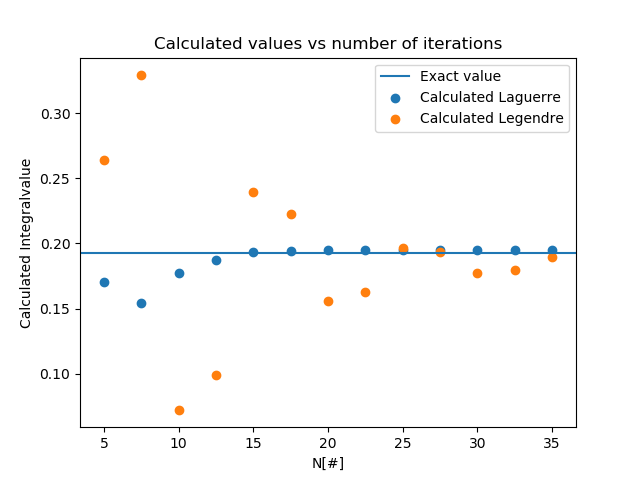
\includegraphics[width=200px]{Leg_lag_int.png}
			\caption{: Calculated values of the integral against number of iterations using Gauss-Legendre and Gauss-Laguerre.}
			\label{fig:int}
	\end{center}
	\end{figure}

	\begin{table}[h!]
		\caption{: Integration using Gauss-Legendre, varying N, with $\lambda=3$ }
			\label{Tab: Legendre}
		\begin{tabular}{c c c c}
			N & Result & Diff. from exact & Time used (s)\\
			\hline
			10 & 0.071980 & 0.120785  & 0.113204\\
			15 & 0.239088 & 0.046323  & 1.299465\\
			20 & 0.156139 & 0.036626  & 7.389662\\
			25 & 0.196817 & 0.003052  & 28.340030\\
			27 & 0.193524 & 0.000759  & 44.707851\\
			30 & 0.177283 & 0.015482  & 87.724024\\
		\end{tabular}
	\end{table}

	\begin{table}[h!]
		\caption{: Integration using Gauss-Laguerre, variying N}
		\begin{tabular}{c c c c}
			N & Result & Diff. from exact & Time used (s)\\
			\hline
			10 & 0.177081 & 0.015684 & 0.072103\\
			15 & 0.193285 & 0.000520 & 0.871607\\
			20 & 0.194786 & 0.002021 & 4.997395\\
			25 & 0.194804 & 0.002039 & 20.496292\\
			27 & 0.193524 & 0.002030 & 31.343583\\
			30 & 0.194779 & 0.002014 & 60.214597\\
		\end{tabular}
		\label{Tab: Laguerre}
	\end{table}

	\begin{figure}[hbt]
	\begin{center}
			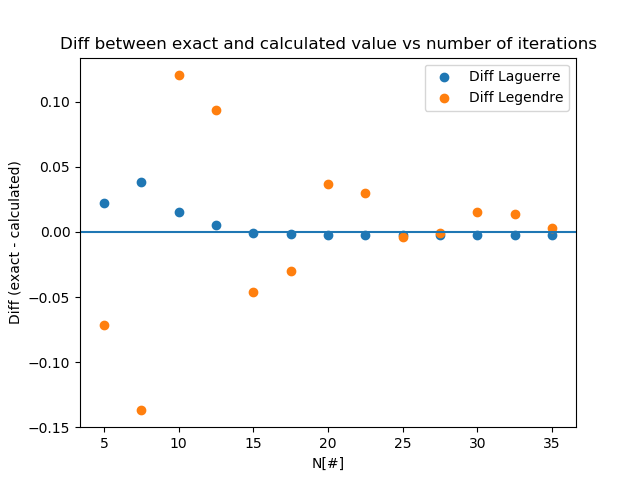
\includegraphics[width=200px]{Leg_lag_diff.png}
			\caption{: Difference from the exact value of the integral for Gauss-Legendre and Gauss-Laguerre against number of iterations.}
			\label{fig:diff}
	\end{center}
	\end{figure}

	The brute force Monte Carlo-method results are presented in table \ref{Tab: MC}. Our improved and adapted Monte Carlo-method results are presented in table \ref{Tab: improvedMC}.

	\begin{table}[h!]
		\caption{: Integration using Monte Carle integration, variying N}
		\label{Tab: MC}
		\begin{tabular}{c c c c}
			N & Result & Diff. from exact & Time used (s) \\
			\hline
			$10^5$ & 0.244992 & 0.052227 & 0.00665 \\
			$10^6$ & 0.183088 & 0.009676 & 0.06485 \\
			$10^7$ & 0.193923 & 0.001159 & 0.66153 \\
			$10^8$ & 0.192657 & 0.000108 & 6.49192 \\
		\end{tabular}
	\end{table}

	\begin{table}[h!]
		\caption{: Integration using imporoved Monte Carle integration, variying N}
		\begin{tabular}{c c c c c}
			N & Result & Diff. from exact & Time used (s) & Time used when parallelized (s) \\
			\hline
			$10^5$ & 0.192894 & 0.000129 & 0.0139 & 0.0093 \\
			$10^6$ & 0.193056 & 0.000291 & 0.1406 & 0.0939 \\
			$10^7$ & 0.193333 & 0.000568 & 1.3990 & 0.9992 \\
			$10^8$ & 0.193324 & 0.000049 & 13.993 & 9.9839 \\
		\end{tabular}
		\label{Tab: improvedMC}
	\end{table}


\section*{Discussion}
	The Gauss-Legendre quadrature is a brute force method, and we can see from our results that is is not a very precise method. We had to try with different integration limits in order to test which limits that gave the best results. Increasing the number of mesh points above, $N = 27$ actually resulted in a less precise approximation, which was unexpected.\\

	By changing to spherical coordinates, we avoid approximating infinity in 4 of the 6 dimenisions of the integral, and lets us use the Gauss-Laguerre quadrature. In this method, we got better results overall, and increasing the number of mesh points improved the precision up to a point, where the precision remained almost constant. We got the best result for $N=15$, resulting in a difference of $5.02\cdot10^{-4}$ from the exact value.

	The results for the Monte Carlo integration is found in \ref{Tab: MC} and \ref{Tab: improvedMC}. When the results were analyzed, we observed that the integral was different every time the program was run. This was expected, because we are generating random numbers with a new seed every time we ran the program. Beause of this, we ran the program several times and found the average of those integrals. This gave us reliable results to analyze.
	The results show that the standard, brute force, Monte Carlo method is a relatively poor method, not presenting a satisfying result even with $10^8$ random points. Our improved Monte Carlo integration, however, gave precise, satisfying results with only $10^5$ integration points. Strangely, though, $10^6$ and $10^7$ gave increasingly imprecise results, while $10^8$ yielded a more precise result than all the above, although taking 100 times longer than $10^5$.

	Additionally, we can see that parallelization slightly improves the running time of the improved Monte Carlo method, but not by a factor 4, which is the number of cores in the computer that ran the program, which is what we would expect.

\section*{Conclusion}
	Our results show that the brute force ways of numerically approximating our integral are unsatisfactory and not precise enough. When we account for and specialize our methods to our integrand and the integral limits, allowing us to use Laguerre polynomials or an exponential distribution, and spherical coordinates, we get much more precise results with fewer mesh points for the Gaussian quadrature and fewer random points in the Monte Carlo method.

	Overall, comparing the results of the Gaussian quadrature using Laguerre-polynomials to the improved Monte Carlo method, we see that both give reasonably precise results, but the Gaussian method doesn't continue to improve by increasing the number of mesh points, while the improved Monte Carlo method seems to improve with an increasing number of integration points.

	Time-wise, it would seem like the [] method is more efficient than the other methods, giving better precision faster. It is also easy to parallelize, improving both precision and speed.

\section*{Bibliography}
	\href{https://github.com/emmernme/MENA-Compfys/tree/master/Project3}{Link to our GitHub repository.}

\end{document}
